\documentclass{article}
%\usepackage{comment}
\usepackage{amsmath}
%\usepackage{xargs}
\usepackage{physics}
\usepackage{graphicx}
%\usepackage{todonotes}
%\usepackage[pdftex,dvipsnames]{xcolor}
\usepackage[labelfont=bf]{caption}
\usepackage{hyperref}
\newcommand{\mb}[1]{\mathbf{#1}}
\usepackage[T1]{fontenc}
\usepackage[utf8]{inputenc}
\usepackage{xcolor}
\definecolor{textblue}{rgb}{.2,.2,.7}
\definecolor{textred}{rgb}{0.54,0,0}
\definecolor{textgreen}{rgb}{0,0.43,0}
\usepackage{listings}
\lstset{language=Python, 
numbers=left, 
numberstyle=\tiny, 
stepnumber=1,
numbersep=5pt, 
tabsize=4,
basicstyle=\ttfamily,
keywordstyle=\color{textblue},
commentstyle=\color{textred},   
stringstyle=\color{textgreen},
frame=none,                    
columns=fullflexible,
keepspaces=true,
xleftmargin=\parindent,
showstringspaces=false}
\usepackage{multicol}

\begin{document}
\title{Fort-BPsym Documentation}
\author{Adam Duster}
\date{\today\\v1.0}
\maketitle
\begin{abstract}
	Fort-BPsym is a program that takes geometry information about a molecule from an existing HDF5 file, generates the Behler-Parinello radial and angular symmetry functions for the geometries, and writes the results to a new HDF5 file.
\end{abstract}
\tableofcontents
\section{Introduction}
	Fort-BPsym is a program that takes geometry information about existing molecules, generates the Behler-Parinello (BP) radial and angular symmetry functions for the geometries, and writes the results to a new HDF5 file. Symmetry function vectors "scan" cartesian space for the presence of specific elements and can be used as input to a neural network.
	
	Elements of the symmetry function vector correspond to scanning for elements at a specific radius from the $i$-th atom or the presence of a specific combination of elements at a given angle, called radial and angular basis functions respectively.
 The number of angular and basis functions can be increased to an arbitrary value, increasing the resolution of the input vector at the cost of exponentially increasing the computational expense of training and evaluating the network, as well as increasing the number of parameters of the system. 
 
	The symmetry functions used are the
\section{Usage}
\subsection{Installation and Execution}
In order to install the program, you must first compile or install the HDF5 file library. On CentOS, the command is 

\texttt{yum install hdf5-devel}

On Ubuntu:

\texttt{apt install libhdf5-dev}

Then add the location of the library to the \texttt{LD\_LIBRARY\_PATH} variable or edit the makefile with the location of the installed library. Next do the following

\texttt{cd src}

\texttt{make all}

The executable should be compiled and ready to run by typing:

\texttt{./gen\_symfunc\_parallel [input\_hdf5.h5] [output\_hdf5.h5]}

\subsection{Testing the program}
The program can be tested by executing the following commands from the program root directory:

\texttt{cd test\_files}

\texttt{cd test\_parallel}

\texttt{./test.sh}

The testing script should compile the program, and run it to generate the the output file \texttt{./2\_waters-symfuncs.h5} from the input file

\texttt{./test\_files/2\_water\_clusters.h5}.

 It will then call the script \texttt{./test\_files/compare\_basis\_functions.py} to compare the elements of the newly generated basis functions with the file \texttt{./test\_files/reference.h5}. The script will output whether the reference elements are bigger, smaller, or equal to the newly generated one.
 
\subsection{Input HDF5 Structure}
This program requires the hdf5 file to have the folowing as top-level datasets. Note that max-atoms is a parameter that should be the same between all of the datasets and the dimensions are in row-major order (so should be backwards if this file is to be created by a FORTRAN program).


\begin{tabular}{| l | l | p{5.1cm} |}
\hline
Dataset Name & Type & Description \\
\hline
\texttt{atomic\_number} & \texttt{int\*1} & The atomic numbers of the atoms. Dimensions should be (num-geoms, max-atoms). \\
\texttt{cartesian\_coordinates} & real*8 & The cartesian coordinates in $\mathrm{\AA}$. Should have dimensions of (num-geoms, max-atoms, 3). \\
\texttt{num\_atoms} & int*2 & The number of atoms for a given geometry. Should have dimensions of (num-geoms). \\
\hline
\end{tabular}

\subsection{Output HDF5 Structure}
The program currently outputs the following hdf5 datasets. Note that the dimensions for each file are given in row major order and thus must be inverted for use with FORTRAN programs:

\begin{tabular}{|l | p{7.0cm} |}
\hline
\texttt{o\_radial\_sym\_funcs} & Oxygen radial symmetry function vector. Should have dimensions of (number of oxygens in all geometries, 48 = number of radial basis elements) \\ \hline
\texttt{h\_radial\_sym\_funcs} & Hydrogen radial symmetry function vector. Should have dimensions of (number of hydrogens in all geometries, 48 = number of radial basis elements) \\ \hline
\texttt{h\_angular\_sym\_funcs} & Hydrogen angular symmetry function vector. Should have dimensions of (number of hydrogens in all geometries, 36 = number of radial basis elements) \\ \hline
\texttt{o\_angular\_sym\_funcs} & Oxygen angular symmetry function vector. Should have dimensions of (number of hydrogens in all geometries, 54 = number of radial basis elements) \\ \hline
\texttt{o\_mol\_index} & Key for linking basis function indices with a given molecule. This should have dimensions of (number of geometries, 2) For example, in a file which contains the symmetry function vectors for two geometries with 6 hydrogens in each geometry, this dataset would contain the following array: [[0, 3],[3, 6]] indicating that the rows 0, 1, and 2 belong to the first molecule and that rows 3, 4, and 5 belong to the second. \\ \hline
\texttt{h\_mol\_index} & See above \\
\hline
\end{tabular}

\subsection{Basis vector layout}
In the current implementation, the program has a fixed layout for the basis vectors. The used bond and angle types and the order of the types in this implementation are:

\begin{center}
\begin{tabular}{| l | c |}
\hline
O bond & (H, O) \\
H bond & (H, O) \\
O angle & ([O, O], [H, O], [H, H]) \\
H angle & ([H, H], [H, O])\\
\hline
\end{tabular} 
\end{center}

As each bond type is described by 24 $\eta$ and $R_s$ parameters, this means that the oxygen symmetry function vector (has length of 48 for given atom) will have the first 24 elements devoted to the O-H bond and the last 24 elements to the O-O bond. This is the same for the angles. The $\eta$ and $R_s$ parameters for each bond type are as follows:

\begin{multicols}{3}
\begin{tabular}{| r | c | c |}
\hline
\# & $\eta$ & $R_s$ \\ 
\hline
 1  &   0.800  &  19.531  \\
 2  &   1.113  &  10.090  \\
 3  &   1.426  &   6.146  \\
 4  &   1.739  &   4.133  \\
 5  &   2.052  &   2.968  \\
 6  &   2.365  &   2.234  \\
 7  &   2.678  &   1.743  \\
 8  &   2.991  &   1.397  \\
 9  &   3.304  &   1.145  \\
10  &   3.617  &   0.955  \\
11  &   3.930  &   0.809  \\
12  &   4.243  &   0.694  \\
13  &   4.557  &   0.602  \\
14  &   4.870  &   0.527  \\
15  &   5.183  &   0.465  \\
16  &   5.496  &   0.414  \\
17  &   5.809  &   0.370  \\
18  &   6.122  &   0.334  \\
19  &   6.435  &   0.302  \\
20  &   6.748  &   0.275  \\
21  &   7.061  &   0.251  \\
22  &   7.374  &   0.230  \\
23  &   7.687  &   0.212  \\
24  &   8.000  &   0.195  \\
\hline
\end{tabular}

\begin{tabular}{| r | c | c | c |}
\hline
\# & $\eta`$ & $\zeta$ & $\lambda$ \\  \hline
 1  &  0.001  &   1  &  -1 \\
 2  &  0.001  &   1  &   1 \\
 3  &  0.001  &   4  &  -1 \\
 4  &  0.001  &   4  &   1 \\
 5  &  0.001  &  16  &  -1 \\
 6  &  0.001  &  16  &   1 \\
 7  &  0.010  &   1  &  -1 \\
 8  &  0.010  &   1  &   1 \\
 9  &  0.010  &   4  &  -1 \\
10  &  0.010  &   4  &   1 \\
11  &  0.010  &  16  &  -1 \\
12  &  0.010  &  16  &   1 \\
13  &  0.050  &   1  &  -1 \\
14  &  0.050  &   1  &   1 \\
15  &  0.050  &   4  &  -1 \\
16  &  0.050  &   4  &   1 \\
17  &  0.050  &  16  &  -1 \\
18  &  0.050  &  16  &   1 \\
\hline 
\end{tabular}
\end{multicols}

\subsection{Creating an HDF5 File}
While any program can be used to create the input HDF5 file, one can be generated with a helper script included at the following location:

 \texttt{./scripts/xyz2hdf5.py}
 
 Instructions are included at the beginning of the script
 
\section{Symmetry Function Definitions}

\subsection{Input Vectors}
Elements of the symmetry vector correspond to scanning for elements at a specific radius from the $i$-th atom or the presence of a specific combination of elements at a given angle, called radial and angular basis functions respectively.
 The number of angular and basis functions can be increased to an arbitrary value, increasing the resolution of the input vector at the cost of exponentially increasing the computational expense of training and evaluating the network, as well as increasing the number of parameters of the system. 
 A radial basis function has the following expression:
\begin{equation}\label{eq:rad}
	G^{1}_{i} = \sum_{j \neq i}^{all} e^{-\eta ( R_{ij} - R_{s})^2} f_{c}(R_{ij})
\end{equation}
where $R_s$ is the distance to scan, $R_{ij}$ is the distance between the $i$-th and $j$-th atom, $\eta$ is a parameter controlling the width of the gaussian function, and $f_c(R_{ij})$ is the smoothing function:
\begin{equation}
 	f_c(R_{ij}) = 
	\begin{cases}
		\frac{1}{2}\left[\cos{(\frac{\pi R_{ij}} {R_s})} + 1 \right] & for R_{ij} \leq R_{c} \\
		0 & for R_{ij} > R_c

	\end{cases}
\end{equation}
In this expression, $R_{ij}$ is the distance between the $i$-th and the $j$-th atom nad $R_c$ is a parameter which represents the cutoff distance for the symmetry functions.The cutoff function is necessary to ensure that the basis functions do not change abruptly when atoms enter the largest distance that is to be scanned. It smoothly and monotonically decreases to 0 as $R_ij$ approaches $R_s$.

The angular symmetry functions describe the angular distribution of two atom types surrounding a given atom by the following expression:
\begin{equation}\label{eq:angnotused}
	G_i^2 = 2^{1 - \zeta} \sum_{j,k \neq i}^{all} ( 1 + \lambda \cos{\theta_{ijk}}) ^\zeta e^{-\eta` ( R_{ij}^2 + R_{ik}^2 + R_{jk}^2)} f_c (R_{ij}) f_c(R_{ik}) f_c(R_{jk})
\end{equation}
OR:
\begin{equation}\label{eq:ang}
	G_i^2 = 2^{1 - \zeta} \sum_{j,k \neq i}^{all} ( 1 + \lambda \cos{\theta_{ijk}}) ^\zeta e^{-\eta` ( R_{ij} + R_{ik} + R_{jk})^2} f_c (R_{ij}) f_c(R_{ik}) f_c(R_{jk})
\end{equation}
Here, $\theta$ is the angle formed by the vectors from the $i$-th to the $j$-th and $i$-th to the $k$-th atoms, $\lambda$ is a parameter used to invert the  cosine function, $\eta `$ is a parameter used to control the gaussian width, and $\zeta$ increases the specificity of the basis function for the given angle. While both of these equation appear in the literaure, following citation TODO from 2018, we will use equation\eqref{eq:ang}.

For each atom, a predetermined number of radial and symmetry functions must be selected and the symmetry function parameters do not change throughout the course of the NN weight optimization.
 For the proton transfer through water exeperiment proposed later, the symmetry functions will be based on ref and include 24 radial Gaussian-shape filters, with $R_s$ values distributed evenly between $0.8 \mathrm{\AA}$ and $8.0 \mathrm{\AA}$.
 The width of the associated $eta$ parameter will be proportional to the center's position by the expression $1/\sqrt{2\eta} = 0.2 R_s$. The angular probe will use $\zeta = \left[ 1, 4, 16 \right]$ for the filter widths, $\lambda = \left[ -1, 1 \right]$ for switching the filter's center between 0 and $\pi$, and $\eta` = \left[ 0.001, 0.01, 0.05\right] (\mathrm{\AA}^{-2})$ for the levels of separation dependence. This will yield a feature of length 82 for H atoms, and 100 for O. The effect of changing the parameters for the radial and angular basis functions are shown in  \ref{fig:rad_funcs} and \ref{fig:ang_funcs} respectively. Note that panel D is currently how the radial symmetry functions are implemented.
\begin{figure}
	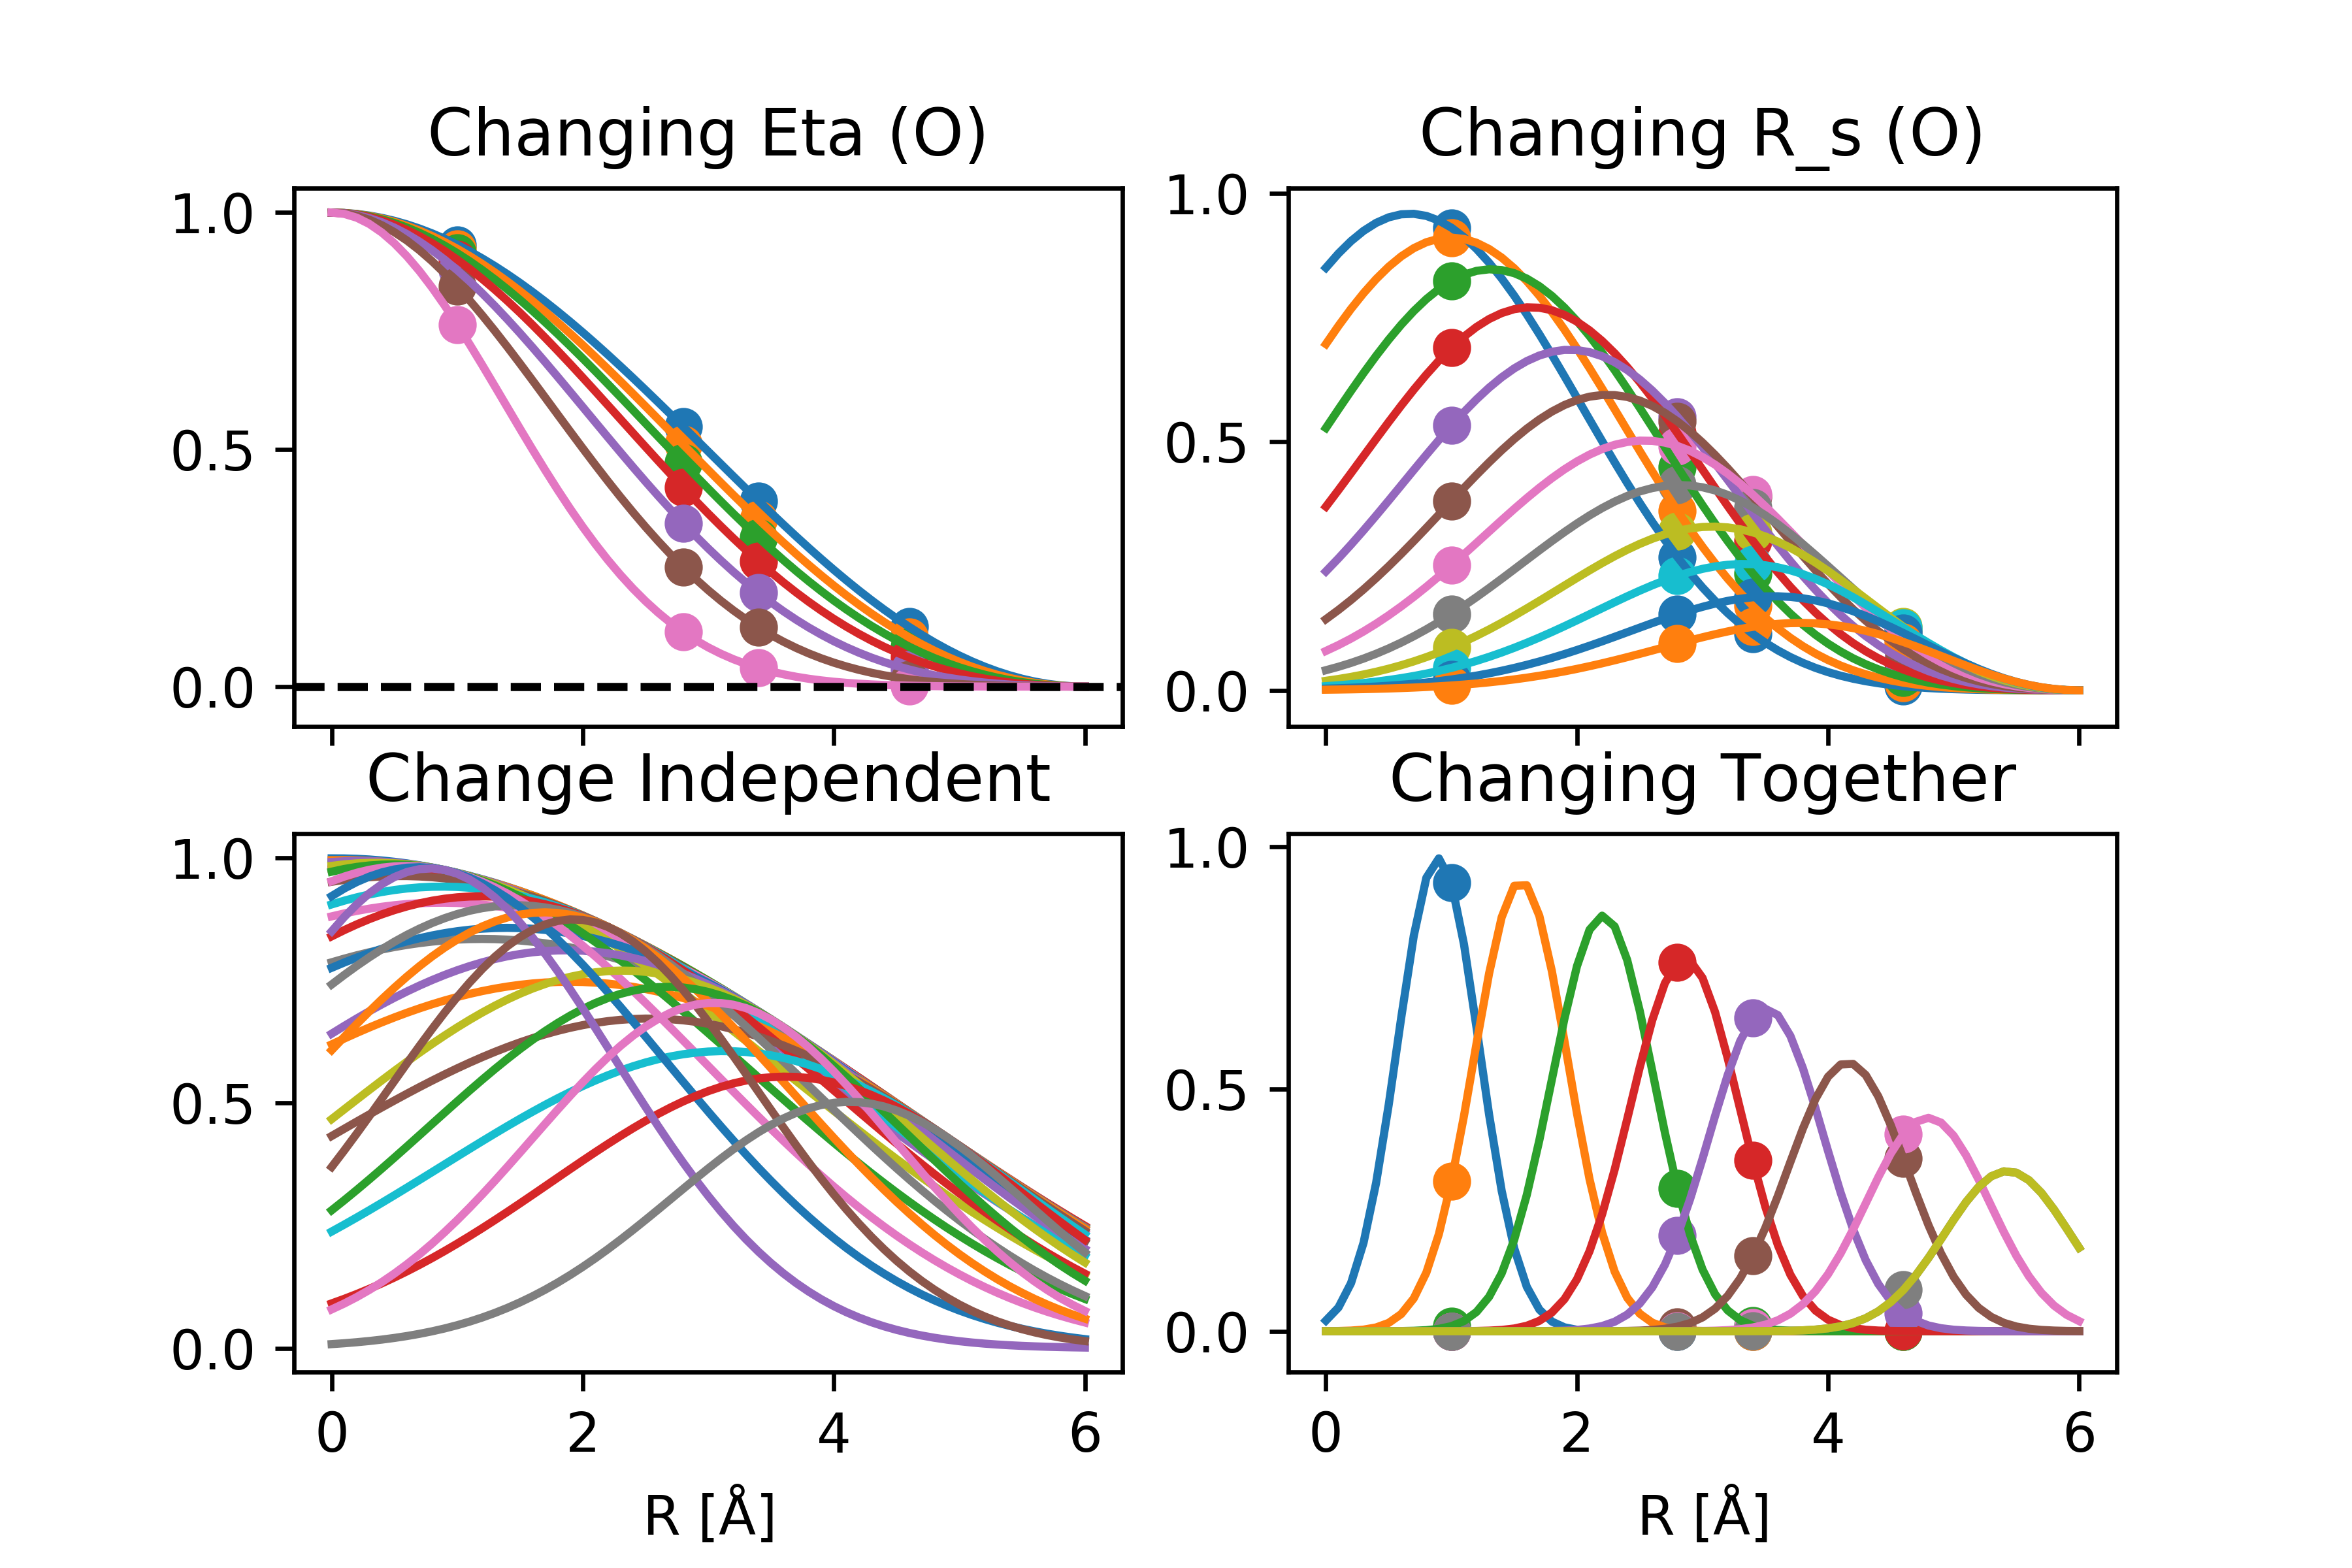
\includegraphics[width=\linewidth]{./img/rad_graphs.png}	\caption{Changes in radial basis function while adjusting parameters. The colored points represent the value of the symmetry function for an atom located at R $\mathrm{\AA}$ away from the given atom.}
	\label{fig:rad_funcs}
\end{figure}
\ref{fig:ang_funcs}
\begin{figure}
	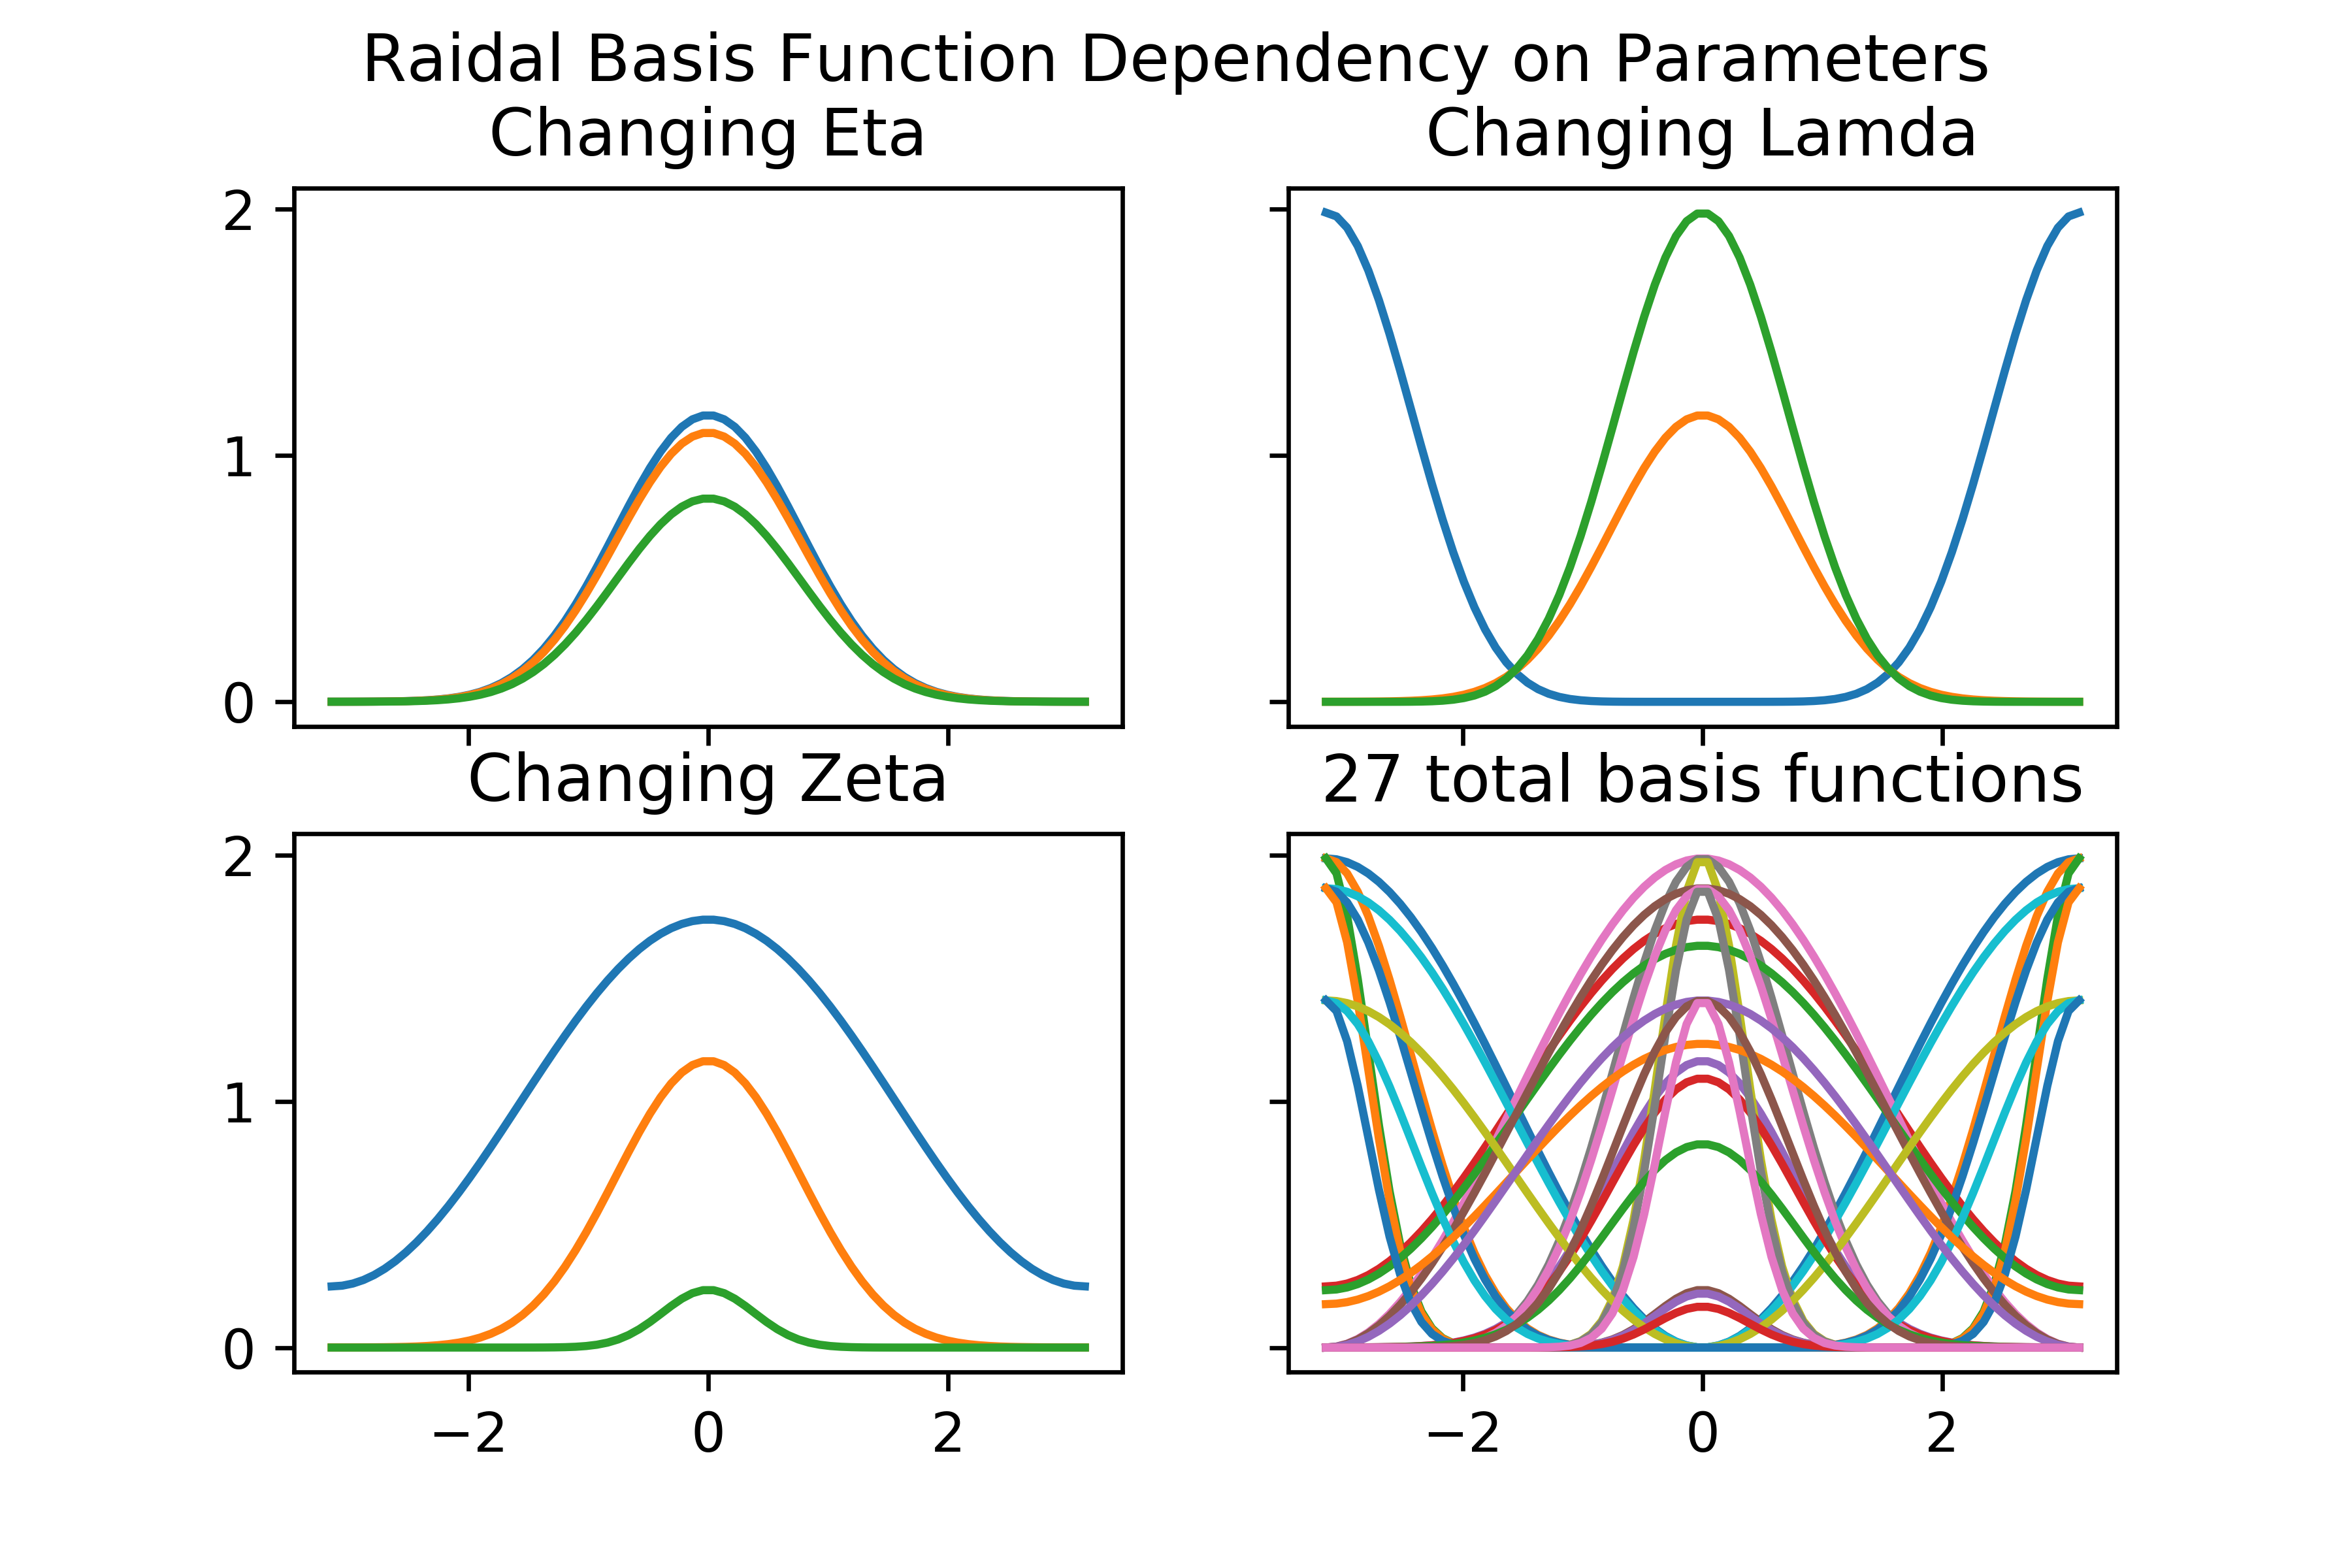
\includegraphics[width=\linewidth]{./img/ang_graphs.png}	\caption{Changes in angular basis function while adjusting parameters. The colored points represent the value of the symmetry function for an atom located at R $\mathrm{\AA}$ away from the given atom. This needs to be checked to ensure that equation 4 was used}
	\label{fig:ang_funcs}
\end{figure}
\newpage
\subsection{Symmetry Function Gradient}
The gradients of the symmetry function terms are presented here in order of increasing complexity.

The gradient of the distance $R_{ij}$ with respect to $i$ is the unit vector along the line between the two points:

\begin{equation}
\frac{\partial R_{ij}}{\mb{X}_{i}} = -\frac{\mathbf{X}_j-\mathbf{X}_i}{\lVert \mathbf{X}_j - \mathbf{X}_i \rVert} = -\frac{\mathbf{X}_j-\mathbf{X}_i}{R_{ij}}
\end{equation}

\begin{equation}
\frac{d R_{ij}}{d \mb{X}_{j}} = - \frac{\partial R_{ij}}{\partial\mb{X}_{i}}
\end{equation}

The gradient of the smoothing function with respect to the ${i}$-th cartesian coordinate:
\begin{equation}
\frac{\partial f_c (R_{ij}) } { \mb{X}_{i}} = -\frac{\pi}{2 
 \mathrm{R_s}}  \sin ( \frac{\pi R_{ij}}{\mathrm{R_s}}) \frac{\partial R_{ij}}{\mb{X}_{i}}
\end{equation}

The gradient of the $j$-th component of the $i$-th radial symmetry function:
\begin{equation}\label{eq:rad_derivative}
\frac{\partial G_{i,j}^2 } { \partial \mb{X}_i} = e^{-\eta ( R_{ij} - \mathrm{R_s} )^2} \left[ -2 \eta ( R_{ij} - \mathrm{R_s} )  f_c (R_{ij}) \frac{\partial R_{ij}}{\partial  \mb{X}_i} + \frac{\partial f_c ( R_{ij} )}{\partial \mb{X}_i} \right] 
\end{equation}

\subsubsection{Angular Symmetry Functions}

The angular symmetry function terms and gradients.

\begin{equation}
\frac{\partial } {\partial \mb{X}_i}
 e^{-\eta ` \left( R_{ij} + R_{ik} + R_{jk} \right)^2 } =
  -2 \eta` \left( R_{ij} + R_{ik} + R_{jk} \right) e^{-\eta` \left( R_{ij} + R_{ik} + R_{jk} \right)^2   } \left(
\frac{d R_{ij}}{\partial \mb{X}_i} + \frac{d R_{ik}}{\partial \mb{X}_i} \right)
\end{equation}

\begin{equation}
\frac{\partial } {\partial \mb{X}_i} ( 1 + \lambda \cos{\theta_{ijk}} )^\zeta  = \zeta ( 1 + \lambda \cos \theta_{ijk} ) ^ {\zeta - 1} \lambda\frac{\partial \cos \theta_{ijk} } {\partial \mb{X}_i}
\end{equation}

As $\cos \theta$ can be expressed as:

\begin{equation}
\cos \theta_{ijk} = \frac{\mb{R}_{ij} \cdot  \mb{R}_{ik}} { R_{ij}  R_{ik}}
\end{equation}

Here, the gradient with respect to $\mb{X}_j$ or $\mb{X}_k$ is:

\begin{equation}
\frac{\partial \cos \theta_{ijk} } {\partial \mb{X}_j} = -\frac{\cos{\theta}}{R_{ij}} \frac{\partial R_{ij}}{\partial \mb{X}_j} + \frac{\mb{R}_{ik}}{R_{ij} R_{ik}}
\end{equation}

The gradient with respect to $\mb{X}_i$ is:
%\begin{equation}
%\frac{\partial \cos \theta_{ijk} } {\partial \mb{X}_i} = -\frac{\mb{R}_{ij} \cdot \mathbf{R}_{ik}  }{ \left( R_{ij}  R_{ik} \right) ^ 2}  
%\left( R_{ik} \frac{\partial R_{ij} } {\partial \mb{X}_i} + R_{ij} \frac{\partial R_{ik} } {\partial \mb{X}_i} \right) + \frac{ 2\mb{X}_i - \mb{X}_j - \mb{X}_k} { R_{ij} R_{ik} }
%\end{equation}

\begin{equation}
\frac{\partial \cos \theta_{ijk} } {\partial \mb{X}_i} = -\frac{\cos{\theta}  }{  R_{ij}  R_{ik} }  
\left( R_{ik} \frac{\partial R_{ij} } {\partial \mb{X}_i} + R_{ij} \frac{\partial R_{ik} } {\partial \mb{X}_i} \right) + \frac{ 2\mb{X}_i - \mb{X}_j - \mb{X}_k} { R_{ij} R_{ik} }
\end{equation}

This is implemented as and equivalent to:
\begin{equation}
\frac{\partial \cos \theta_{ijk} } {\partial \mb{X}_i} = - \frac{\partial \cos \theta_{ijk} } {\partial \mb{X}_j} - \frac{\partial \cos \theta_{ijk} } {\partial \mb{X}_k}
\end{equation}

\section{Tests}
\subsection{Test 1 - Comparing answers with reference}
\subsection{Test 2 - Calculation of the radial gradient}
In this test, a simple system was constructed to check the numerical accuracy of the gradient calculations. The O-H molecule was constructed, with the O-H bond measuring 1.0 $\mathrm{\AA}$ and lying along the $x$-axis. The $y$ and $z$ coordinates were all set to 0. Thus, the derivative of the radial symmetry functions should only be non-zero in the $x$ direction, and the result can be easily checked. Additionally, the gradient should be symmetrical between the O and the H atoms.The answers are presented here. The ith atom is the O with coordinates of (-1, 0, 0| and the jth atom is the H with coordinates (1, 0, 0).


$\eta = 19.53125$

$\mathrm{R_s} = 0.8$

$\frac{\partial R_{ij}}{\partial x} = 1$

$\frac{\partial f_c (R_{ij}) } { \partial x} = - \frac{\pi}{2 * 0.8} sin \left( \frac {\pi}{0.8} \right) * 1 $

From equation \eqref{eq:rad_derivative}, the final answer can be calculated:

$\frac{\partial G^2_{ij}}{\partial x} = -3.475089$


\end{document}
